\PassOptionsToPackage{naturalnames}{hyperref}
\RequirePackage{luatex85}
\documentclass{article}
\usepackage{geometry}
%\usepackage{fullpage}
\usepackage{parskip}
\usepackage{physics}
\usepackage{amsmath}
\usepackage{amssymb}
\usepackage{xcolor}
\usepackage[colorlinks,linkcolor=blue,citecolor=green]{hyperref}
\usepackage{array}
\usepackage{longtable}
\usepackage{multirow}
\usepackage{comment}
\usepackage{graphicx}
\usepackage{cite}
\usepackage{amsfonts}
\usepackage{bm}
\usepackage{slashed}
\usepackage{dsfont}
\usepackage{mathtools}
\usepackage[compat=1.1.0]{tikz-feynman}
\usepackage{simplewick}
%\usepackage{fourier}
%\usepackage{slashbox}
%\usepackage{intent}
\usepackage{mathrsfs}
\usepackage{xparse}
\usepackage{enumerate}
%\usepackage{axodraw4j}
\usepackage[toc,page]{appendix}


\geometry{left=0.5cm,right=0.5cm,top=1.5cm,bottom=2cm}

\newcommand{\gm}{\gamma^{\mu}}
\newcommand{\gn}{\gamma^{\nu}}
\newcommand{\gs}{\gamma^{\sigma}}
\newcommand{\gr}{\gamma^{\rho}}
\newcommand{\gnr}{g^{\nu\rho}}
\newcommand{\gmr}{g^{\mu\rho}}
\newcommand{\gms}{g^{\mu\sigma}}
\newcommand{\gns}{g^{\nu\sigma}}
\newcommand{\vbp}{\vb{p}}
\newcommand{\vbk}{\vb{k}}
\newcommand{\g}{\gamma}
\renewcommand{\a}{\alpha}
\renewcommand{\b}{\beta}
\renewcommand{\t}{\theta}
\newcommand{\la}{\lambda}
\newcommand{\p}{\phi}
\newcommand{\vp}{\varphi}
\newcommand{\s}{\sigma}
\newcommand{\G}{\Gamma}
\newcommand{\pars}{\slashed\partial}
\newcommand{\ps}{\slashed p}
\newcommand{\ks}{\slashed k}
\newcommand{\lag}{\mathcal{L}}
\newcommand{\da}{^{\dagger}}
\newcommand{\sm}{^{\mu}}
\newcommand{\sn}{^{\nu}}
\newcommand{\smn}{^{\mu\nu}}
\newcommand{\Dm}{D^{\mu}}
\newcommand{\dm}{\partial^{\mu}}
\newcommand{\Asquare}{A^{\mu}A_{\mu}}
\newcommand{\partialsquare}[2]{\partial^{\mu}{#1}\partial_{\mu}{#2}}

\title{Local Operator Divergence}
\author{Yingsheng Huang}
\begin{document}
\maketitle
\section{NRQED local matrix elements}
Since what we what is an operator equation independent of states, we can choose $p^{\mu}=(0,\vb{p})$ as our outstate electron momentum, and put the nucleus on-shell. This way, we can eliminate possible IR divergence and make the integral much easier (especially at NNLO where the first integral will give a $\sinh ^{-1}\left(\frac{1}{\sqrt{\frac{\text{k1}^2}{2 E m}-1}}\right)$ if no constrain condition put at external momentum). 

At NLO: 
\begin{align*}
   \mel{0}{\psi_e(0)N(0)(-ie)\int\dd^4y\bar\psi_e\psi_e A^0(-ie)\int\dd^4z\bar NNA^0}{eN}&=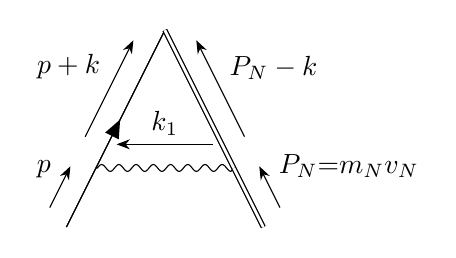
\begin{tikzpicture}[baseline=($(p1)!0.5!(x)$)]
	\begin{feynman}
    \vertex (p1);
	\vertex[right=2.5cm of p1] (p2);
	\vertex at ($(p1)!0.5!(p2)+(0,2.5cm)$) (x) ;
	\vertex at ($(p1)!0.3!(x)$) (y1);
	\vertex at ($(p2)!0.3!(x)$) (z1);
	%
	\diagram* {
	  (p1) -- [fermion] (x);
	  (p2) -- [double distance=1pt] (x);
	  (y1) -- [photon,rmomentum=$k_1$] (z1);
	  (p1) -- [momentum=\(p\)] (y1);
	  (p2) -- [momentum'=$P_{N}\text{=}m_{N}v_{N}$,double distance=1pt] (z1);
	  (y1) -- [momentum=\(p+k\)] (x);
	  (z1) -- [momentum'=\(P_{N}-k\),double distance=1pt] (x);
    };
	\end{feynman}
  \end{tikzpicture}\\
   &=e^2u_N(v_N)\bqty{\int\frac{\dd^3k}{(2\pi)^3}\frac{1}{(\vb{k}-\vb{p})^2(E-\frac{\vb{k}^2}{2m})}(1-\frac{\vb{k}^4}{8m^3(E-\frac{\vb{k}^2}{2m})})}\frac{i}{E-\frac{\vb{p}^2}{2m}}\\
   &
   =-e^2u_N(v_N)[\frac{\pi }{v}+\mathcal{O}(v^2)]\frac{i}{E-\frac{\vb{p}^2}{2m}}
\end{align*}

\clearpage
\begin{appendices}
NRQED matrix element at NLO
\begin{align*}
  &\mel{0}{\psi_e(0)N(0)(-ie)\int\dd^4y\bar\psi_e\psi_e A^0(-ie)\int\dd^4z\bar NNA^0}{eN}=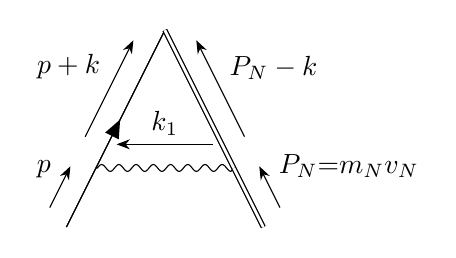
\begin{tikzpicture}[baseline=($(p1)!0.5!(x)$)]
	\begin{feynman}
    \vertex (p1);
	\vertex[right=2.5cm of p1] (p2);
	\vertex at ($(p1)!0.5!(p2)+(0,2.5cm)$) (x) ;
	\vertex at ($(p1)!0.3!(x)$) (y1);
	\vertex at ($(p2)!0.3!(x)$) (z1);
	%
	\diagram* {
	  (p1) -- [fermion] (x);
	  (p2) -- [double distance=1pt] (x);
	  (y1) -- [photon,rmomentum=$k_1$] (z1);
	  (p1) -- [momentum=\(p\)] (y1);
	  (p2) -- [momentum'=$P_{N}\text{=}m_{N}v_{N}$,double distance=1pt] (z1);
	  (y1) -- [momentum=\(p+k\)] (x);
	  (z1) -- [momentum'=\(P_{N}-k\),double distance=1pt] (x);
    };
	\end{feynman}
  \end{tikzpicture}\\
  =&ie^2u_N(v_N)\bqty{\int[\dd k]\frac{1}{\vb{k}^2(-k^0+i\epsilon)(^0+k^0-m-\frac{\vb{(p+k)}^2}{2m}+\frac{\vb{(p+k)}^4}{8m^3}+i\epsilon)}}\frac{i}{E-\frac{\vb{p}^2}{2m}}\\
  =&e^2u_N(v_N)\bqty{\int\frac{\dd^3k}{(2\pi)^3}\frac{1}{(\vb{k}-\vb{p})^2(E-\frac{\vb{k}^2}{2m}+\frac{\vb{k}^4}{8m^3})}}\frac{i}{E-\frac{\vb{p}^2}{2m}}\\
  = &e^2u_N(v_N)\bqty{\int\frac{\dd^3k}{(2\pi)^3}\frac{1}{(\vb{k}-\vb{p})^2(E-\frac{\vb{k}^2}{2m})}(1-\frac{\vb{k}^4}{8m^3(E-\frac{\vb{k}^2}{2m})})}\frac{i}{E-\frac{\vb{p}^2}{2m}}\\
  =&-2me^2u_N(v_N)\frac{i}{E-\frac{\vb{p}^2}{2m}}[\frac{\pi }{2p}+\mathcal{O}(p^2)]
   =-e^2u_N(v_N)\frac{i}{E-\frac{\vb{p}^2}{2m}}[\frac{\pi }{v}+\mathcal{O}(v^2)]
\end{align*}
At NNLO (where we're only interested in divergent parts)
\begin{align*}
  &-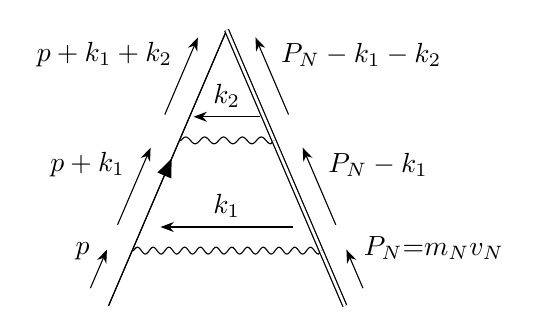
\begin{tikzpicture}[baseline=($(p1)!0.5!(x)$)]
 \begin{feynman}
   \vertex (p1);
 \vertex[right=3cm of p1] (p2);
 \vertex at ($(p1)!0.5!(p2)+(0,3.5cm)$) (x) ;
 \vertex at ($(p1)!0.2!(x)$) (y1);
 \vertex at ($(p2)!0.2!(x)$) (z1);
 \vertex at ($(p1)!0.6!(x)$) (y2);
 \vertex at ($(p2)!0.6!(x)$) (z2);
 %
 \diagram* {
   (p1) -- [fermion] (x);
   (p2) -- [double distance=1pt] (x);
   (y1) -- [photon,rmomentum=$k_1$] (z1);
   (y2) -- [photon,rmomentum=$k_2$] (z2);
   (p1) -- [momentum=\(p\)] (y1);
   (p2) -- [momentum'=$P_{N}\text{=}m_{N}v_{N}$,double distance=1pt] (z1);
   (y1) -- [momentum=\(p+k_1\)] (y2);
   (z1) -- [momentum'=\(P_{N}-k_1\),double distance=1pt] (z2);
   (y2) -- [momentum=\(p+k_1+k_2\)] (x);
   (z2) -- [momentum'=\(P_{N}-k_1-k_2\),double distance=1pt] (x);
   };
 \end{feynman}
 \end{tikzpicture}\\ =&e^4\bqty{\int[dk_1][dk_2]\frac{1}{\vb{\abs{k_1}}^2}\frac{1}{\vb{\abs{k_2}}^2}\frac{1}{-k_1^0-k_2^0+i\epsilon}\frac{1}{-k_1^0+i\epsilon}\frac{1}{p^0+k_1^0-m-\frac{\vb{(p+k_1)}^2}{2m}+i\epsilon}\frac{1}{p^0+k_1^0+k_2^0-m-\frac{\vb{(p+k_1+k_2)}^2}{2m}+i\epsilon}}\frac{i}{E-\frac{\vb{p}^2}{2m}}u_N(v_N)
 \\
 \intertext{do the shift as above}
 =&-e^4\bqty{\int\frac{\dd^3\vb{k_1}}{(2\pi)^3}\frac{\dd^3\vb{k_2}}{(2\pi)^3}\frac{1}{\vb{\abs{k_1-p}}^2}\frac{1}{\vb{\abs{k_2-k_1}}^2}\frac{1}{E-\frac{\vb{\abs{k_1}}^2}{2m}+2i\epsilon}\frac{1}{E-\frac{\vb{\abs{k_2}}^2}{2m}+2i\epsilon}}\frac{i}{E-\frac{\vb{p}^2}{2m}}u_N(v_N)\\
 \intertext{drop $\vb{p}$}
 =&-e^4\bqty{\int\frac{\dd^3\vb{k_1}}{(2\pi)^3}\frac{\dd^3\vb{k_2}}{(2\pi)^3}\frac{1}{\vb{\abs{k_1}}^2}\frac{1}{\vb{\abs{k_2-k_1}}^2}\frac{1}{-\frac{\vb{\abs{k_1}}^2}{2m}+2i\epsilon}\frac{1}{-\frac{\vb{\abs{k_2}}^2}{2m}+2i\epsilon}}\frac{i}{E-\frac{\vb{p}^2}{2m}}u_N(v_N)\\
 \intertext{if we add higher reltivistic correction}
 =&-e^4\bqty{\int\frac{\dd^3\vb{k_1}}{(2\pi)^3}\frac{\dd^3\vb{k_2}}{(2\pi)^3}\frac{1}{\vb{\abs{k_1}}^2}\frac{1}{\vb{\abs{k_2-k_1}}^2}\frac{{2m}}{\vb{\abs{k_1}}^2-\frac{\vb{\abs{k_1}^4}}{4m^2}}\frac{{2m}}{\vb{\abs{k_2}}^2-\frac{\vb{\abs{k_2}^4}}{4m^2}}}\frac{i}{E-\frac{\vb{p}^2}{2m}}u_N(v_N)\\
 =&-4m^2e^4\bqty{\int\frac{\dd^3\vb{k_1}}{(2\pi)^3}\frac{\dd^3\vb{k_2}}{(2\pi)^3}\frac{1}{\vb{\abs{k_1}}^2}\frac{1}{\vb{\abs{k_2-k_1}}^2}\frac{1}{\vb{\abs{k_1}}^2}(1+\frac{\vb{\abs{k_1}^2}}{4m^2})\frac{1}{\vb{\abs{k_2}}^2}(1+\frac{\vb{\abs{k_2}^2}}{4m^2})}\frac{i}{E-\frac{\vb{p}^2}{2m}}u_N(v_N)\\
\end{align*}
The integral (we can verify that $\vb{k}^0$ part is not UV divergent, and we don't care aobut $\vb{k}^8$ term for now) for 
\begin{align*}
  &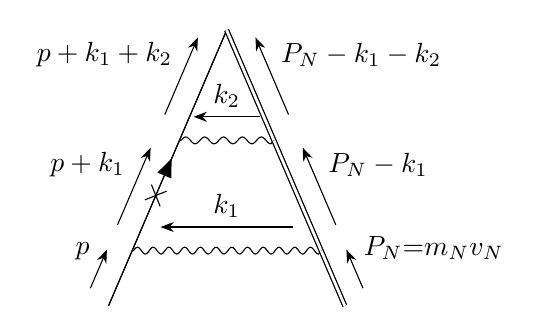
\begin{tikzpicture}[baseline=($(p1)!0.5!(x)$)]
 \begin{feynman}
   \vertex (p1);
 \vertex[right=3cm of p1] (p2);
 \vertex at ($(p1)!0.5!(p2)+(0,3.5cm)$) (x) ;
 \vertex at ($(p1)!0.2!(x)$) (y1);
 \vertex at ($(p2)!0.2!(x)$) (z1);
 \vertex at ($(p1)!0.6!(x)$) (y2);
 \vertex at ($(p2)!0.6!(x)$) (z2);
 \vertex at ($(y1)!0.5!(z1)$) (t);
 %
 \diagram* {
   (p1) -- [fermion] (x);
   (p2) -- [double distance=1pt] (x);
   (y1) -- [photon,rmomentum=$k_1$] (z1);
   (y2) -- [photon,rmomentum=$k_2$] (z2);
   (p1) -- [momentum=\(p\)] (y1);
   (p2) -- [momentum'=$P_{N}\text{=}m_{N}v_{N}$,double distance=1pt] (z1);
   (y1) -- [momentum=\(p+k_1\),insertion=0.5] (y2);
   (z1) -- [momentum'=\(P_{N}-k_1\),double distance=1pt] (z2);
   (y2) -- [momentum=\(p+k_1+k_2\)] (x);
   (z2) -- [momentum'=\(P_{N}-k_1-k_2\),double distance=1pt] (x);
   };
 \end{feynman}
 \end{tikzpicture}=
 \int\frac{\dd^3\vb{k_1}}{(2\pi)^3}\frac{\dd^3\vb{k_2}}{(2\pi)^3}\frac{1}{\vb{\abs{k_1-p}}^2}\frac{1}{\vb{\abs{k_2-k_1}}^2}\frac{\vb{\abs{k_1}}^4/4m^2}{[\vb{\abs{k_1}}^2-2mE]^2}\frac{1}{\vb{\abs{k_2}}^2-2mE}\\
  =&\int_0^1\dd x\int\frac{\dd^3\vb{k_1}}{(2\pi)^3}\frac{1}{\vb{\abs{k_1-p}}^2}\frac{\vb{\abs{k_1}}^4/4m^2}{[\vb{\abs{k_1}}^2-2mE]^2}\frac{\left(\frac{4 \pi }{\Delta_2 }\right)^{2-\frac{d}{2}} \Gamma \left(2-\frac{d}{2}\right)}{(4 \pi )^2 \Gamma (2)}\\
  \intertext{where $\Delta_2=(1-x) \left(\vb{\abs{k_1}}^2 x-2 E m\right)$} 
  =&\frac{1}{(4\pi)^2}\int_0^1\dd x\int\frac{\dd^3\vb{k_1}}{(2\pi)^3}\frac{1}{\vb{\abs{k_1-p}}^2}\frac{\vb{\abs{k_1}}^4/4m^2}{[\vb{\abs{k_1}}^2-2mE]^2}\frac{1}{(\vb{\abs{k_1}}^2-2mE/x)^{2-d/2}}\pqty{\frac{4\pi}{x(1-x)}}^{2-d/2}\Gamma(2-d/2)\\
  =&\frac{1}{(4\pi)^2}\int_0^1\dd x\int_0^1\dd y\dd z\dd t\delta(y+z+t-1)\int\frac{\dd^3 \vb{k_1}}{(2\pi)^3}\frac{zt^{1-d/2}\vb{\abs{k_1}}^4/4m^2}{[\vb{\abs{k_1}}^2+\Delta_1]^{5-d/2}}\frac{\Gamma(5-d/2)}{\Gamma(2-d/2)}\pqty{\frac{4\pi}{x(1-x)}}^{2-d/2}\Gamma(2-d/2)\\
  \intertext{where $\Delta_1=y(1-y)\vb{p}^2-2mE(z+t/x)$}
  =&\frac{1}{4m^2(4\pi)^2}\int_0^1\dd x\int_0^1\dd y\dd z\dd t\delta(y+z+t-1)zt^{1-d/2}\frac{d (d+2)}{4}\frac{\Gamma \left(3-d\right)}{(4 \pi )^{3-d/2} } \left(\frac{4 \pi }{\Delta_1 }\right)^{3-d} \pqty{\frac{4\pi}{x(1-x)}}^{2-d/2}\\
  =&-\frac{1}{128 \pi ^2 (d-3) m^2}+\text{finite terms}
\end{align*}
\begin{align*}
  &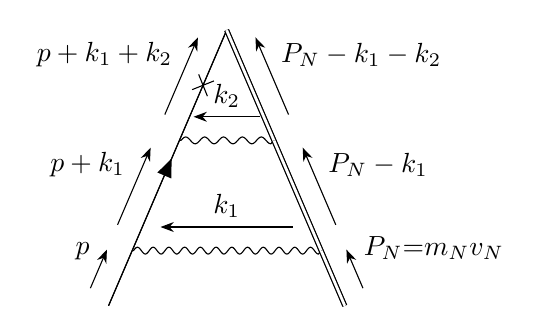
\begin{tikzpicture}[baseline=($(p1)!0.5!(x)$)]
 \begin{feynman}
   \vertex (p1);
 \vertex[right=3cm of p1] (p2);
 \vertex at ($(p1)!0.5!(p2)+(0,3.5cm)$) (x) ;
 \vertex at ($(p1)!0.2!(x)$) (y1);
 \vertex at ($(p2)!0.2!(x)$) (z1);
 \vertex at ($(p1)!0.6!(x)$) (y2);
 \vertex at ($(p2)!0.6!(x)$) (z2);
 \vertex at ($(y1)!0.5!(z1)$) (t);
 %
 \diagram* {
   (p1) -- [fermion] (x);
   (p2) -- [double distance=1pt] (x);
   (y1) -- [photon,rmomentum=$k_1$] (z1);
   (y2) -- [photon,rmomentum=$k_2$] (z2);
   (p1) -- [momentum=\(p\)] (y1);
   (p2) -- [momentum'=$P_{N}\text{=}m_{N}v_{N}$,double distance=1pt] (z1);
   (y1) -- [momentum=\(p+k_1\)] (y2);
   (z1) -- [momentum'=\(P_{N}-k_1\),double distance=1pt] (z2);
   (y2) -- [momentum=\(p+k_1+k_2\),insertion=0.5] (x);
   (z2) -- [momentum'=\(P_{N}-k_1-k_2\),double distance=1pt] (x);
   };
 \end{feynman}
 \end{tikzpicture}=
   \int\frac{\dd^3\vb{k_1}}{(2\pi)^3}\frac{\dd^3\vb{k_2}}{(2\pi)^3}\frac{1}{\vb{\abs{k_1-p}}^2}\frac{1}{\vb{\abs{k_2-k_1}}^2}\frac{1}{\vb{\abs{k_1}}^2-2mE}\frac{\vb{\abs{k_2}}^4/4m^2}{[\vb{\abs{k_2}}^2-2mE]^2}\\
  =&\frac{1}{4m^2}\int_0^1\dd x\int\frac{\dd^3\vb{k_1}}{(2\pi)^3}\frac{1}{\abs{\vb{k_1-p}}^2}\frac{1}{\vb{\abs{k_1}}^2-2mE}\frac{(1-x)\Gamma(1-d/2)}{8\pi}\pqty{\frac{4\pi}{\Delta_2}}^{1-d/2}\frac{d(d+2)}{4}\\
  \intertext{where $\Delta_2=x(1-x)\vb{\abs{k_1}}^2-2mE(1-x)$}
  =&\frac{1}{4m^2}\int_0^1\dd x\int_0^1\dd y\dd z\dd t\frac{t^{-d/2}}{[\vb{\abs{k_1}}^2+\Delta_1]^{3-d/2}}\frac{\Gamma{(3-d/2)}}{\Gamma{(1-d/2)}}\delta(y+z+t-1)\frac{\Gamma(1-d/2)}{8\pi}\pqty{\frac{4\pi}{x(1-x)}}^{1-d/2}\frac{d(d+2)x}{4}\\
  \intertext{where $\Delta_1=y(1-y)\vb{p}^2-2mEz-2mE\frac{t}{x }$}
  =&\frac{1}{4m^2}\int_0^1\dd x\int_0^1\dd y\dd z\dd t\delta(y+z+t-1)\frac{1}{(4\pi)^{3-d/2}} \left(\frac{4 \pi }{\Delta_1 }\right)^{3-d} \frac{\Gamma \left(3-d\right)}{8\pi}\pqty{\frac{4\pi}{x(1-x)}}^{1-d/2}\frac{d(d+2)x}{4}t^{-d/2}\\
  =&\frac{15}{8192 \pi ^2 (d-3) m^2}+\text{finite terms}
\end{align*}
Check the contour integral
\begin{align*}
  &-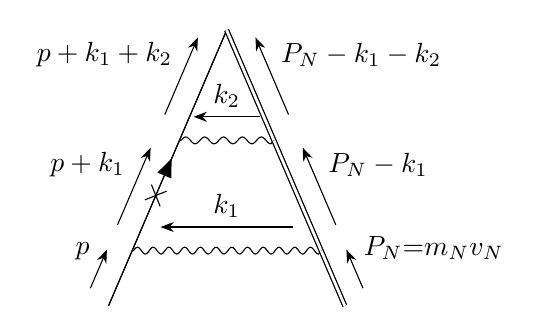
\begin{tikzpicture}[baseline=($(p1)!0.5!(x)$)]
 \begin{feynman}
   \vertex (p1);
 \vertex[right=3cm of p1] (p2);
 \vertex at ($(p1)!0.5!(p2)+(0,3.5cm)$) (x) ;
 \vertex at ($(p1)!0.2!(x)$) (y1);
 \vertex at ($(p2)!0.2!(x)$) (z1);
 \vertex at ($(p1)!0.6!(x)$) (y2);
 \vertex at ($(p2)!0.6!(x)$) (z2);
 \vertex at ($(y1)!0.5!(z1)$) (t);
 %
 \diagram* {
   (p1) -- [fermion] (x);
   (p2) -- [double distance=1pt] (x);
   (y1) -- [photon,rmomentum=$k_1$] (z1);
   (y2) -- [photon,rmomentum=$k_2$] (z2);
   (p1) -- [momentum=\(p\)] (y1);
   (p2) -- [momentum'=$P_{N}\text{=}m_{N}v_{N}$,double distance=1pt] (z1);
   (y1) -- [momentum=\(p+k_1\),insertion=0.5] (y2);
   (z1) -- [momentum'=\(P_{N}-k_1\),double distance=1pt] (z2);
   (y2) -- [momentum=\(p+k_1+k_2\)] (x);
   (z2) -- [momentum'=\(P_{N}-k_1-k_2\),double distance=1pt] (x);
   };
 \end{feynman}
 \end{tikzpicture}\\ =&e^4\bqty{\int[dk_1][dk_2]\frac{1}{\vb{\abs{k_1}}^2}\frac{1}{\vb{\abs{k_2}}^2}\frac{1}{-k_1^0-k_2^0+i\epsilon}\frac{1}{-k_1^0+i\epsilon}\frac{(\vb{p+k})^4/8m^3}{[p^0+k_1^0-m-\frac{\vb{(p+k_1)}^2}{2m}+i\epsilon]^2}\frac{1}{p^0+k_1^0+k_2^0-m-\frac{\vb{(p+k_1+k_2)}^2}{2m}+i\epsilon}}\frac{i}{E-\frac{\vb{p}^2}{2m}}u_N(v_N)\\
 =&-e^4\bqty{\int\frac{\dd^3\vb{k_1}}{(2\pi)^3}\frac{\dd^3\vb{k_2}}{(2\pi)^3}\frac{1}{\vb{\abs{k_1-p}}^2}\frac{1}{\vb{\abs{k_2-k_1}}^2}\frac{\vb{\abs{k_1}}^4/8m^3}{[E-\frac{\vb{\abs{k_1}}^2}{2m}+2i\epsilon]^2}\frac{1}{E-\frac{\vb{\abs{k_2}}^2}{2m}+2i\epsilon}}\frac{i}{E-\frac{\vb{p}^2}{2m}}u_N(v_N)
\end{align*}
which is the same as previous (by expansion) one.

Contact (Darwin) term
\begin{align*}
  -&\bqty{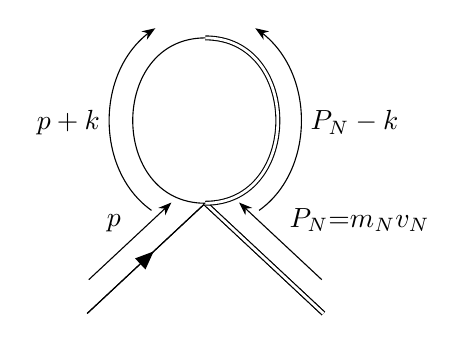
\begin{tikzpicture}[baseline=($(p1)!0.5!(x)$)]
 \begin{feynman}
   \vertex (p1);
 \vertex[right=3cm of p1] (p2);
 \vertex at ($(p1)!0.5!(p2)+(0,3.5cm)$) (x) ;
 \vertex at ($(p1)!0.4!(x)+(0.9cm,0)$) (i);
% \vertex[above=0.05cm of x] (text) {\(0\)};
 %
 \diagram* {
   (p1) -- [fermion] (i);
   (p2) -- [double distance=1pt] (i);
   (p1) -- [momentum=\(p\)] (i);
   (p2) -- [momentum'=$P_{N}\text{=}m_{N}v_{N}$,double distance=1pt] (i);
   (i) -- [momentum=\(p+k\), half left] (x);
   (i) -- [momentum'=\(P_{N}-k\),double distance=1pt, half right] (x);
   };
 \end{feynman}
\end{tikzpicture}+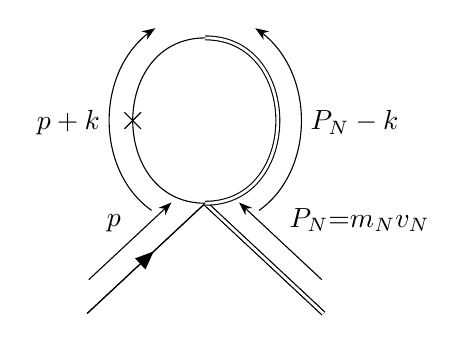
\begin{tikzpicture}[baseline=($(p1)!0.5!(x)$)]
 \begin{feynman}
   \vertex (p1);
 \vertex[right=3cm of p1] (p2);
 \vertex at ($(p1)!0.5!(p2)+(0,3.5cm)$) (x) ;
 \vertex at ($(p1)!0.4!(x)+(0.9cm,0)$) (i);
% \vertex[above=0.05cm of x] (text) {\(0\)};
 %
 \diagram* {
   (p1) -- [fermion] (i);
   (p2) -- [double distance=1pt] (i);
   (p1) -- [momentum=\(p\)] (i);
   (p2) -- [momentum'=$P_{N}\text{=}m_{N}v_{N}$,double distance=1pt] (i);
   (i) -- [momentum=\(p+k\), half left,insertion=0.5] (x);
   (i) -- [momentum'=\(P_{N}-k\),double distance=1pt, half right] (x);
   };
 \end{feynman}
\end{tikzpicture}}\\=&\frac{4\pi e^4}{3m}\bqty{\int\frac{\dd^4 k}{(2\pi)^4}\frac{1}{p^0+k^0-m-\frac{(\vb{p+k})^2}{2m}+i\epsilon}\pqty{1+\frac{\vb{(p+k)}^4/8m^3}{p^0+k^0-m-\frac{(\vb{p+k})^2}{2m}+i\epsilon}}\frac{1}{-k^0+i\epsilon}}\frac{i}{E-\frac{\vb{p}^2}{2m}}u_N(v_N)
\\
=&\frac{4\pi e^4}{3m}\bqty{\int\frac{\dd^3\vb{k}}{(2\pi)^3}\frac{1}{E-\frac{\vb{k}^2}{2m}+2i\epsilon}\pqty{1+\frac{\vb{\abs{k}}^4/8m^3}{E-\frac{\vb{k}^2}{2m}+i\epsilon}}}\frac{i}{E-\frac{\vb{p}^2}{2m}}u_N(v_N)
\\
\intertext{if the dispersion relation is up to $\vb{k}^4$ then}&=\frac{4 e^4m}{3}
\end{align*}




\end{appendices}

\end{document}
